\documentclass[10pt,twocolumn]{IEEEtran11}
\usepackage{algpseudocode}
\usepackage{times}
\usepackage{cite}
\usepackage{epsfig}
\usepackage[T1]{fontenc}
\usepackage{graphicx}
\usepackage{subfigure}
\def\BibTeX{{\rm B\kern-.05em{\sc i\kern-.025em b}\kern-.08em
    T\kern-.1667em\lower.7ex\hbox{E}\kern-.125emX}}

\oddsidemargin -15pt
\evensidemargin -15pt
\leftmargin 0 pt
\topmargin -30pt
\textwidth = 6.9 in
\textheight = 9.0 in
\makeatletter
\newcommand{\removelatexerror}{\let\@latex@error\@gobble}
\makeatother
\newcommand{\itembase}{\setlength{\itemsep}{0pt}}
\newcommand{\eg}{{\it e.g., }}
\newcommand{\ie}{{\it i.e., }}
\graphicspath{{figs/}}

\begin{document}
%\input{psfig.sty}
\bibliographystyle{IEEE}

\title{\Large \bf Title
%\thanks{
}
\author{
Peter McKay\\
Computer and Information Science Department\\
University of Oregon\\
{\em pem@cs.uoregon.edu}
}
\maketitle
% You have to do this to suppress page numbers.  Don't ask.
%\pagestyle{empty}
\begin{abstract}
In this paper, we consider the problem of automatic forest coverage 
classification, as posed by the Kaggle competition: 
``Forest Cover Type Prediction.''  In short, we use python's machine 
learning libraries to construct a model capable of reliably predicting 
the predominant type of tree cover for a small region of forest, given 
a collection of cartographic variables. We create such a model by 
leveraging a voting body of a number of different classifiers, with a 
second layer of classifiers for certain cases.  We optimize this 
technique by carrying out a number of feature transformations and 
subsequent feature scaling operations, making use of a number of 
statistical relationships discovered through judicious application of 
graphical data analysis tools.

We find that the classifier thus developed is capable of reliably 
predicting accurate forest cover with approximately 80\% accuracy.  In 
reviewing the particulars of the performance of our algorithms, we 
gain some insight into the data set, and the problem domain in general.\\

\end{abstract}
%%% Local Variables: 
%%% mode: latex
%%% TeX-master: "main"
%%% End: 


\begin{keywords} 
Machine Learning, Forestry
\end{keywords}



\section{Introduction}
\label{sec:-intro}

Education sometimes seems like a process of ever-increasing 
specialization. Preschool acclimatizes larval humans to basic
scholarly etiquette (listening, sharing, naptime) grade-school begins 
to separate learning into a number of different subjects, and by the 
time college rolls around one is expected to pick a major.  By the time 
one has reached the PhD program, one's course of study has narrowed 
down to a small tunnel of the unknown, sometimes just a single problem.

When dealing with questions on the frontiers of science, it is not 
uncommon to encounter as problem that falls within the purview of many
such narrow fields, necessitating the addition of more and more team 
members.  This is something a problem, because, as any software engineer 
can tell you\cite{mythical}, throwing more people at a problem is not 
exactly a solution.  Despite how interested our University 
Administration seems in the subject, interdisciplinary research 
just doesn't seem to scale very well.

One of the real draws for machine learning lies in allowing us to 
compartmentalize our need for understanding, avoiding issues by 
transforming our problems into a familiar domain and extracting 
the answers we need.  So long as our model ``understands'' a problem, 
we can ignore a certain level of complexity and move on to the 
solving the interest parts of the problem.  This allows a computer 
scientist with an aversion to the so-called ``outdoors'' to make a 
number of correct judgments about forests, all from the comfort of 
their office.

From our limited experiences in the outdoors, we can make a few judgments about
the construct of a forest given a few data points. An accomplished expert 
in the fields of ecology or geography, specializing in the climate of 
that forest, might be able to tell us quite a bit more information based 
on that same starting data.  In the noble tradition of computer science, we 
would like to avoid doing that much work, and we will apply machine 
learning techniques to accomplish this task.  To that end, we consider 
the following multiclass classification problem. We construct a 
classifier that, when presented with a number of cartographic variables 
that apply to a 30--30 meter cell of forest, classifies such a cell by 
the predominant type of tree cover found therein.

In this paper, we utilize a multi-level ensemble method of 
classification.  We add a number of new features, scale the feature 
vector appropriately, and then train a collection of different 
classifiers on that data.  The classifiers vote to determine the 
classification of an example, and in some cases, pass on that vote into 
another layer of machines trained on a smaller subset of the training 
data.  We accomplish these tasks using Python and a series of libraries 
designed for data analysis and machine learning.  In so doing, our model 
reaches approximately 80\% accuracy on the Kaggle data set. 






\begin{table}
  \begin{tabular}{ l | r }
    \hline
    Elevation & Elevation in meters \\
    \hline
    Aspect & Aspect in degrees azimuth \\
    \hline
    Slope & Slope in degrees \\
    \hline
    Horizontal\_Distance\_To\_Hydrology & Meters to nearest water-body \\
    \hline
    Vertical\_Distance\_To\_Hydrology & Meters to nearest water-body \\
    \hline
    Horizontal\_Distance\_To\_Roadways & Meters to nearest roadway \\
    \hline
    Hillshade\_9am (0 to 255 index) & Hillshade index at 9am \\
    \hline
    Hillshade\_Noon (0 to 255 index) & Hillshade index at noon \\
    \hline
    Hillshade\_3pm (0 to 255 index) & Hillshade index at 3pm \\
    \hline
    Horizontal\_Distance\_To\_Fire\_Points & Meters, wildfire ignition points \\
    \hline
    Wilderness\_Area & Wilderness area designation \\
    \hline
    Soil\_Type & Soil Type designation \\
    \hline
  \end{tabular}
  \caption{Feature List}
  \label{table:featurelist}
\end{table}



%%% Local Variables: 
%%% mode: latex
%%% TeX-master: "main"
%%% End: 

\section{Background}
\label{sec:-back}
\subsection{Problem Structure}
The forest coverage classification problem clearly fits into the 
category of a multiclass classification problem, in which we describe 
a classifier that maps from a feature vector to one of a series of 
possible output labels.  This feature vector, as outlined in table 
\ref{table:featurelist}, contains a mix of continuous and discrete 
values.  The discrete features, as visualized in figures \ref{fig:soil} 
and \ref{fig:wilderness}, account for multiclass features encoded with 
the one-hot encoding method.  

Given these features, we wish to classify our example with a choice 
from the labels 
below:
\begin{enumerate}
\item Spruce/Fir
\item Lodgepole Pine
\item Ponderosa Pine
\item Cottonwood/Willow
\item Aspen
\item Douglas-fir
\item Krummholz
\end{enumerate}

Unlike a binary classifier, it is quite easy to end up with an 
error rate well over 50\% when dealing with a multiclass 
classifier.  As we're dealing data collected from a natural source, we 
expect we will find a high degree of noise within the data set.


\begin{figure*}
\centering
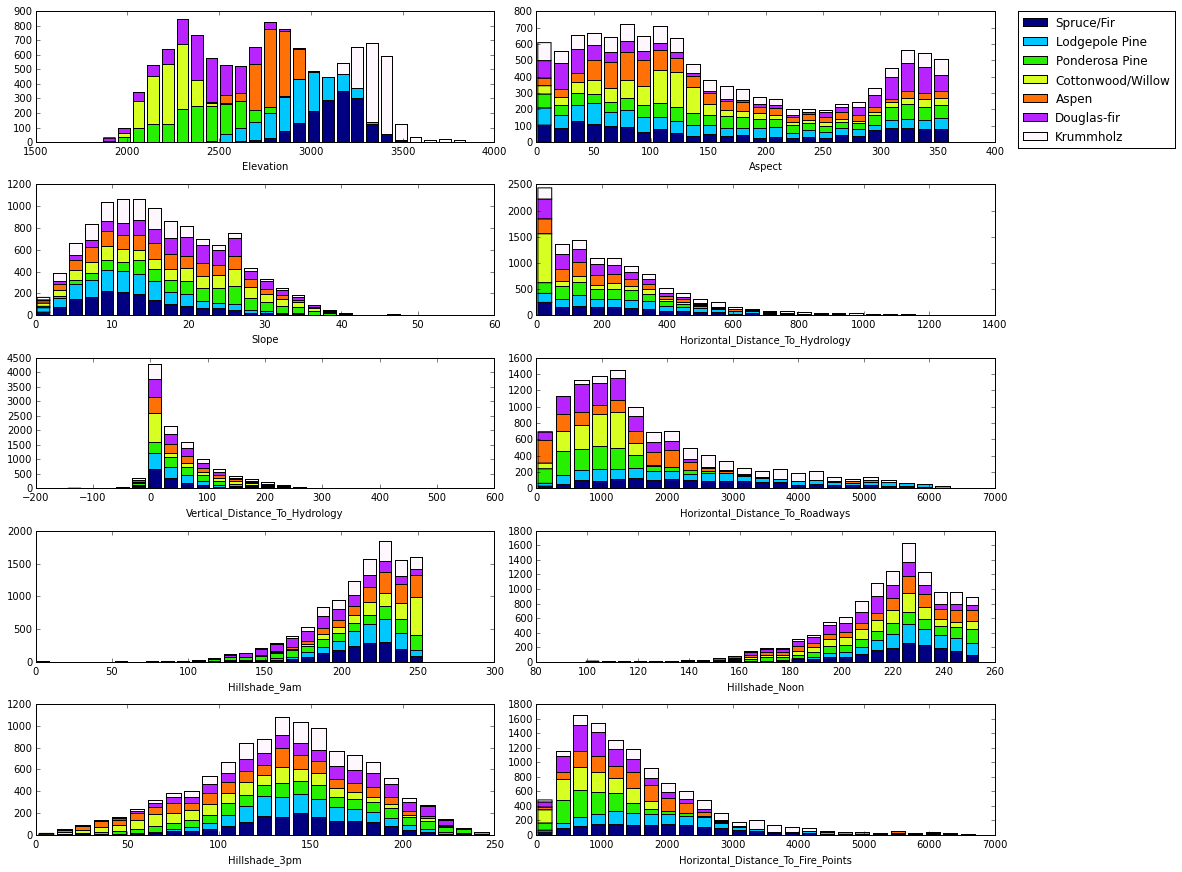
\includegraphics[width=\linewidth]{continuous}
 \caption{Continuous variables}
 \label{fig:continuous_features}
\end{figure*}

\begin{figure*}
\centering
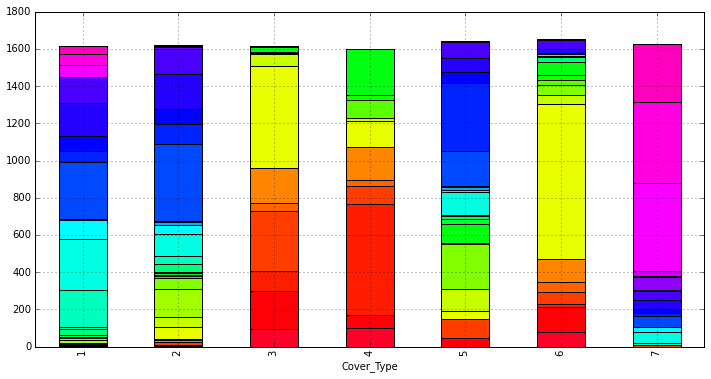
\includegraphics[width=\linewidth]{soil_type}
 \caption{Soil types and accompanying cover types}
 \label{fig:soil}
\end{figure*}

\begin{figure*}
\centering
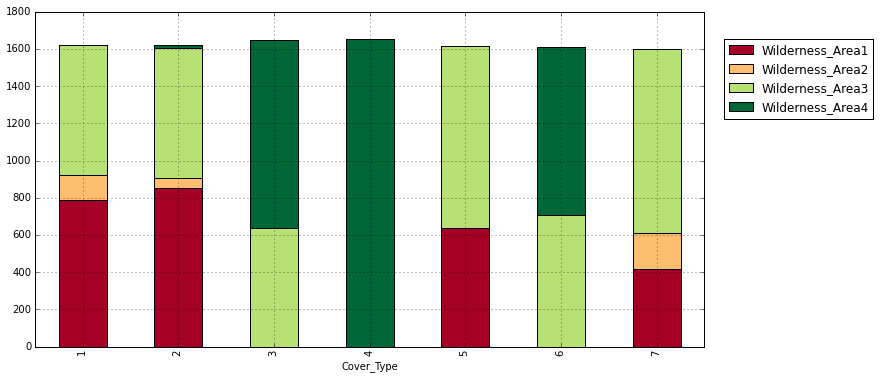
\includegraphics[width=\linewidth]{wilderness}
 \caption{Wilderness types and accompanying cover types}
 \label{fig:wilderness}
\end{figure*}

\subsection{Solution}
The classification solution we assemble to solve this problem involves 
a number of different machine learning models.  We began the project by 
attempting a Random Forest classifier, but eventually expanded to also 
make use of a Gradient Boost Machine, a Support Vector Machine, and a 
k-Nearest Neighbor classifier.  Each of these machines has its own 
strengths and weaknesses, which we will discuss as follows.  Each model 
has a number of hyperparameters that must be tuned properly before 
evaluating the total efficacy of such a technique: we will cover the 
tuning process in the following sections.

A Random Forest classifier\cite{breiman2001random} is an example of an 
ensemble method, a sort of mashup of decision trees with a machine 
learning technique called bootstrap aggregating, or, more colloquially, 
bagging\cite{bagging}.  Instead of constructing a single tree on the 
entirety of the training set, Random Forest constructs many smaller 
trees on randomly selected subsets of the training data.  This has a 
number of perks: Random Forests are resistant to artifacts of training 
set ordering and are highly robust in the face of noise and superfluous 
features.  Perhaps most importantly, Random Forests, by effectively 
averaging together a number of decision trees, can effectively mitigate 
the tendency of decision trees to overfit the training data.  As a 
small bonus, the structure of the algorithm allows for efficient 
parallelism, making this a very quick algorithm on a computer with 
sufficient cores.

When we began exploring the idea of adding further classifiers, we 
settled on the Grading Boosting Machine\cite{gbm} after some small 
amount of testing.  Like Random Forest, GBM is an ensemble method that 
constructs a number of subsidiary decision trees.  In this case, the 
algorithm combines decision trees with the idea of 
boosting\cite{boosting}.  Boosting is, in abstract, the process of 
combining a number of poor predictors into a single good predictor.  
In the case of a tree-based GBM, our process is superficially similar 
to bagging, insofar as we create trees based on repeatedly selecting 
subsets from the total training set.  The difference lies primarily in 
how we weight such trees.  Instead of relying largely on the sheer mass 
of trees, we instead attempt to select subtrees that will improve 
currently weak areas of the aggregate predictor.

k-Nearest Neighbor\cite{nearest} is arguably the simplest algorithm we 
deploy in the course of this paper.  We consider an n-dimensional 
graph (for a total of n features) over the feature space.  By populating 
the graph with our training examples, our predictor takes the form of 
simply checking the class of the k training examples that are closest 
to the testing instance.  This distance metric can be a simple 
Euclidean distance calculation, or one of a number of more complex 
metrics suited for particular problem domains.

Support Vector Machines\cite{support} share some commonalities with 
the k-NN algorithm as described above.  We repeat the process of 
populating an n-dimensional graph with training examples, and from 
there the algorithms diverge significantly.  


Most of the algorithms we made use of for this classification problem 
were provided by scikit-learn, with a couple of important exceptions.  
When mixing our classifiers together into a voting body, we rolled our 
own method of voting.  In addition, the confusion matrix as detailed in 
figure \ref{fig:confusion} motivated a second layer of Random Forest 
classifier, where certain classes of classifications cause our system to 
double-check its work.  


%%% Local Variables: 
%%% mode: latex
%%% TeX-master: "main"
%%% End: 

\section{Methodology}
\label{sec:-method}

\subsection{}
\subsection{}
%%% Local Variables: 
%%% mode: latex
%%% TeX-master: "main"
%%% End: 

\section{Results}
\label{sec:-res}



%%% Local Variables: 
%%% mode: latex
%%% TeX-master: "main"
%%% End: 

\section{Conclusion}
\label{sec:-conc}

In this paper, we examine a number of machine learning algorithms as 
they apply to the problem of classifying forest cover based on 
cartographic variables.  We specify accuracy both for naive solutions 
(before tuning), and for solutions with more carefully tuned 
hyperparameters.  The final collection of k-Nearest Neighbor, Support 
Vector Machine, Gradient Boosting Machine, and Random Forest result in 
a significant increase in accuracy over the next best approach, at a 
final accuracy of 80\%.

In the course of our experimentation, we discovered a number of 
interesting relationships between the variables in the feature set.  
If we had the opportunity to undertake future work on this project, we 
would like to undertake a more comprehensive and formal analysis of the 
data.  For instance, what kind of relationship exists between the 
vairous Hillshade values?  How closely correlated are they with 
Elevation?  We have a great many soil types, but some of them seem to 
overlap. Do all soil types classified as ``extremely stony'' occur with 
similar environments, regardless of whether the soil is Bross family or 
Leighcan-Moran family?  We would be interested in answering these 
questions and more, perhaps in conjunction with an actual expert in 
the domain of geology.






%%% Local Variables: 
%%% mode: latex
%%% TeX-master: "main"
%%% End: 


\section{Acknowledgments}


%\small
\bibliography{citations}
\end{document}
